% Options for packages loaded elsewhere
\PassOptionsToPackage{unicode}{hyperref}
\PassOptionsToPackage{hyphens}{url}
%
\documentclass[
]{book}
\usepackage{amsmath,amssymb}
\usepackage{iftex}
\ifPDFTeX
  \usepackage[T1]{fontenc}
  \usepackage[utf8]{inputenc}
  \usepackage{textcomp} % provide euro and other symbols
\else % if luatex or xetex
  \usepackage{unicode-math} % this also loads fontspec
  \defaultfontfeatures{Scale=MatchLowercase}
  \defaultfontfeatures[\rmfamily]{Ligatures=TeX,Scale=1}
\fi
\usepackage{lmodern}
\ifPDFTeX\else
  % xetex/luatex font selection
\fi
% Use upquote if available, for straight quotes in verbatim environments
\IfFileExists{upquote.sty}{\usepackage{upquote}}{}
\IfFileExists{microtype.sty}{% use microtype if available
  \usepackage[]{microtype}
  \UseMicrotypeSet[protrusion]{basicmath} % disable protrusion for tt fonts
}{}
\makeatletter
\@ifundefined{KOMAClassName}{% if non-KOMA class
  \IfFileExists{parskip.sty}{%
    \usepackage{parskip}
  }{% else
    \setlength{\parindent}{0pt}
    \setlength{\parskip}{6pt plus 2pt minus 1pt}}
}{% if KOMA class
  \KOMAoptions{parskip=half}}
\makeatother
\usepackage{xcolor}
\usepackage{longtable,booktabs,array}
\usepackage{calc} % for calculating minipage widths
% Correct order of tables after \paragraph or \subparagraph
\usepackage{etoolbox}
\makeatletter
\patchcmd\longtable{\par}{\if@noskipsec\mbox{}\fi\par}{}{}
\makeatother
% Allow footnotes in longtable head/foot
\IfFileExists{footnotehyper.sty}{\usepackage{footnotehyper}}{\usepackage{footnote}}
\makesavenoteenv{longtable}
\usepackage{graphicx}
\makeatletter
\def\maxwidth{\ifdim\Gin@nat@width>\linewidth\linewidth\else\Gin@nat@width\fi}
\def\maxheight{\ifdim\Gin@nat@height>\textheight\textheight\else\Gin@nat@height\fi}
\makeatother
% Scale images if necessary, so that they will not overflow the page
% margins by default, and it is still possible to overwrite the defaults
% using explicit options in \includegraphics[width, height, ...]{}
\setkeys{Gin}{width=\maxwidth,height=\maxheight,keepaspectratio}
% Set default figure placement to htbp
\makeatletter
\def\fps@figure{htbp}
\makeatother
\setlength{\emergencystretch}{3em} % prevent overfull lines
\providecommand{\tightlist}{%
  \setlength{\itemsep}{0pt}\setlength{\parskip}{0pt}}
\setcounter{secnumdepth}{5}
\usepackage{booktabs}
\usepackage{amsthm}
\makeatletter
\def\thm@space@setup{%
  \thm@preskip=8pt plus 2pt minus 4pt
  \thm@postskip=\thm@preskip
}
\makeatother

\usepackage{tcolorbox}
\tcbuselibrary{breakable}

\newtcolorbox{blackbox}{
  colback=black,
  coltext=white,
  colframe=black,
  boxsep=5pt,
  arc=4pt,
  breakable
  }
\newtcolorbox{bonus}{
  colback=blue!15,
  colframe=blue!15,
  coltext=black!80,
  boxsep=5pt,
  arc=4pt,
  breakable
  }
\newtcolorbox{reflect}{
  colback=green!5,
  colframe=green!5,
  coltext=black!80,
  boxsep=5pt,
  arc=4pt,
  breakable
  }
\newtcolorbox{assessment}{
  colback=blue!5,
  colframe=blue!5,
  coltext=black!80,
  boxsep=5pt,
  arc=4pt,
  breakable
  }
  
\newtcolorbox{progress}{
  colback=purple!10,
  colframe=purple!10,
  coltext=black!80,
  boxsep=5pt,
  arc=4pt,
  breakable
  }
\newtcolorbox{video}{
  colback=yellow!5,
  colframe=yellow!5,
  coltext=black!80,
  boxsep=5pt,
  arc=4pt,
  breakable
  }
\newtcolorbox{caution}{
  colback=red!5,
  colframe=red!5,
  coltext=black!80,
  boxsep=5pt,
  arc=4pt,
  breakable
  }
\newtcolorbox{feedback}{
  colback=black!5,
  colframe=black!5,
  coltext=black!80,
  boxsep=5pt,
  arc=4pt,
  breakable
  }
\ifLuaTeX
  \usepackage{selnolig}  % disable illegal ligatures
\fi
\usepackage[]{natbib}
\bibliographystyle{apalike}
\IfFileExists{bookmark.sty}{\usepackage{bookmark}}{\usepackage{hyperref}}
\IfFileExists{xurl.sty}{\usepackage{xurl}}{} % add URL line breaks if available
\urlstyle{same}
\hypersetup{
  pdftitle={Introduction to Psychology},
  pdfauthor={Todd Dutka},
  hidelinks,
  pdfcreator={LaTeX via pandoc}}

\title{Introduction to Psychology}
\author{Todd Dutka}
\date{}

\begin{document}
\maketitle

{
\setcounter{tocdepth}{1}
\tableofcontents
}
\hypertarget{welcome}{%
\chapter*{Welcome}\label{welcome}}
\addcontentsline{toc}{chapter}{Welcome}

This is the course book for {[}insert{]}. This book is divided into 6 units of study to help you engage with the materials. The course resources and learning activities are designed not only to help prepare you for the course assessments, but also to give you opportinities to practice various skills.

Below you will find information about how to navigate this book. Please also refer the schedule in Moodle, as well as the Asseessment section in Moodle for instructions on required readings and assignments.

\hypertarget{course-notes}{%
\section*{Course Notes}\label{course-notes}}
\addcontentsline{toc}{section}{Course Notes}

You should be reading this information in the context of a Trinity Western University course offered via Moodle. If this is not the case, then this may be an unauthorized reproduction of the course. Please contact \href{mailto:elearning@twu.ca}{\nolinkurl{elearning@twu.ca}} if you have concerns.

These notes will be your guide through the learning activities and assessment strategies necessary for you to succeed in the course, so it is important for you to engage to the best of your ability and take advantage of the resources available to you through Trinity Western University.

Assessment tasks are managed in other sections of the Moodle course, so be sure to familiarize yourself with those requirements and resources.

\hypertarget{how-this-course-is-built}{%
\section*{How this Course is Built}\label{how-this-course-is-built}}
\addcontentsline{toc}{section}{How this Course is Built}

This course is primarily designed to be completed asynchronously, meaning that there are no scheduled times or places that you are required to meet, even online. You can work according to your own schedule \emph{within the six weeks you have to complete the course}. That said, this is a full university level course and there are timelines that we strongly recommend that you meet to ensure that you are succeeding in building your knowledge through the course.

It would be to your significant disadvantage to submit everything at the end of the course.

Asynchronous courses require learners to be well-organized and self-motivated, and we have included supports for you to help you develop strong learning habits that will ensure your success.

For example, there are several self-check quizzes throughout the course. These quizzes are not graded, but they can be powerful tools for you to ensure you understand key ideas and concepts. We suggest you take each quiz without the aid of your notes and textbook and multiple times until you have mastered the content. This strategy taps into three powerful learning structures that have been shown to be highly effective.

\begin{enumerate}
\def\labelenumi{\arabic{enumi}.}
\tightlist
\item
  \textbf{Effortful recall.} By intentionally trying to recall information without external aids, you are strengthening the neural pathways in your brain that lead to building new connections between ideas. One way to make recall easier is to connect key ideas to other things that you know or have experienced. For example, you might be studying World War II, and you connect the date that Canadians participated in the D-Day operation with something else meaningful to you that happened on June 6, like maybe the date you bought your first car.
\item
  \textbf{Spaced repetition.} By spreading out your attempts on the quiz (leaving a few days between attempts) you can maximize the effects of the first strategy (effortful recall) and ensure that your second or third attempts truly reflect what you know about the topic. We suggest leaving 1-3 days between attempt 1 and 2, then 4-5 days between attempt 2 and 3. You can use a tool like Trello, Notion, or Asana (free versions), or even a task list on your phone to set up a spaced repetition schedule.
\item
  \textbf{Interleaving.} This is the practice of studying a particular topic for a relatively short period of time (maybe 30-40 mins), then switching to a different topic for the same period, before going back to the original topic. We will help build this into your learning by including items from unit 1 in your unit 2-6 quizzes. You can also practice this by taking regular breaks in your work, or even by retaking a unit 1 quiz while you are working in unit 2.
\end{enumerate}

These three strategies are very effective at helping people \emph{remember} key facts about a particular topic, an important first step in learning at the university level. However, you will be asked to do much more than just remember facts. Your ultimate goal is to develop \textbf{evaluative judgement}, or the ability for you to judge for yourself the quality of your (or your peers') responses to prompts.

The discussion forums are a key way for you to do this. We have set up the forums in such a way that you will need to present a response to any given prompt before you see other learners' responses. We strongly encourage you to use this structure to formulate your own ideas before you present them in the forum, and then to use the responses of your peers to help you evaluate your own response.

Using these self-check activities in this way is designed to help you to succeed on the course assignments, upon which your final grade will be determined. These assignments will require you to \textbf{use} the facts of the course to generate unique responses to the prompts, based on your past experiences, knowledge, and ability to evaluate the quality of your own work.

\hypertarget{how-to-navigate-this-book}{%
\subsection*{How To Navigate This Book}\label{how-to-navigate-this-book}}
\addcontentsline{toc}{subsection}{How To Navigate This Book}

To move quickly to different portions of the book, click on the appropriate chapter or section in the table of contents on the left. The buttons at the top of the page allow you to show/hide the table of contents, search the book, change font settings, download a pdf or ebook copy of this book, or get hints on various sections of the book.

\includegraphics{assets/course-intro/menu.png}

The faint left and right arrows at the sides of each page (or bottom of the page if it's narrow enough) allow you to step to the next/previous section. Here's what they look like:

\includegraphics{assets/course-intro/left_arrow.png} 
\includegraphics{assets/course-intro/right_arrow.png}

You can also download an offline copy of this book in various formats, such as pdf or an ebook. If you are having any accessibility or navigation issues with this book, please reach out to your instructor or our online team at \href{mailto:elearning@twu.ca}{\nolinkurl{elearning@twu.ca}}.

\hypertarget{course-units}{%
\subsection*{Course Units}\label{course-units}}
\addcontentsline{toc}{subsection}{Course Units}

This course is organized into 6 units. Each unit of the course will provide you with the following information:

\begin{itemize}
\tightlist
\item
  A general overview of the key concepts that will be addressed during the unit.\\
\item
  Specific learning outcomes and topics for the unit.\\
\item
  Learning activities to help you engage with the concepts. These often include key readings, videos, and reflective prompts.\\
\item
  The Assessment section provides details on assignments you will need to complete throughout the course to demonstrate your understanding of the course learning outcomes.
\end{itemize}

\begin{caution}
Note that assessments, including assignments and discussion posts will be submitted in Moodle. See the Assessment tab in Moodle for the assignment dropboxes.
\end{caution}

\hypertarget{course-activities}{%
\subsection*{Course Activities}\label{course-activities}}
\addcontentsline{toc}{subsection}{Course Activities}

Below is some key information on features you will see throughout the course.~

\begin{reflect}
\textbf{\emph{Learning Activity}}\\
This box will prompt you to engage in course concepts, often by viewing resources and reflecting on your experience and/or learning. Most learning activities are ungraded and are designed to help prepare you for the assessment in this course.
\end{reflect}

\begin{assessment}
\textbf{\emph{Assessment}}\\
This box will signify an assignment or discussion post you will submit in Moodle. Note that these demonstrate your understanding of the course learning outcomes. Be sure to review the grading rubrics for each assignment.
\end{assessment}

\begin{progress}
\textbf{\emph{Checking Your Learning}}\\
This box is for checking your understanding, to make sure you are ready for what follows. Ways to check your learning might include self-check quizzes or questions for discussion. These activities are not graded but are critical for you to be able to begin to develop evaluative judgement in this domain of knowledge.
\end{progress}

\begin{caution}
\textbf{\emph{Note}}\\
This box signifies key notes. It may also warn you of possible problems or pitfalls you may encounter!
\end{caution}

\hypertarget{thought-and-language}{%
\chapter{Thought and Language}\label{thought-and-language}}

\hypertarget{overview}{%
\section*{Overview}\label{overview}}
\addcontentsline{toc}{section}{Overview}

\textbf{\emph{Welcome to Psych 106}}

We begin this course by reviewing some important information on scientific research methodologies. While this review will be self-guided, it is critical that you understand the important elements that constitute valid and reliable scientific research as it is these methodologies that serve as the backbone for psychological studies.

After taking time to review scientific research methodologies, we will turn our attention to the subject of Thought and Language. Developing an understanding of Thought and Language helps us better understand how we think, how we organize our thoughts and our knowledge of the world around us, and how we communicate and act out on this information.

\hypertarget{topics}{%
\subsection*{Topics}\label{topics}}
\addcontentsline{toc}{subsection}{Topics}

This unit is divided into the following topics:

\begin{enumerate}
\def\labelenumi{\arabic{enumi}.}
\tightlist
\item
  Review- Scientific Research\\
\item
  Thinking and Problem Solving\\
\item
  Cognitive Biases\\
\item
  Language and Thought\\
\item
  Animal Language
\end{enumerate}

\hypertarget{learning-outcomes}{%
\subsection*{Learning Outcomes}\label{learning-outcomes}}
\addcontentsline{toc}{subsection}{Learning Outcomes}

When you have completed this unit, you should be able to:

\begin{itemize}
\tightlist
\item
  Define key terminology related to principles of scientific research, research designs, and statistics.\\
\item
  Explain the five characteristics of quality scientific research, and the pros and cons of descriptive, correlational, and experimental research designs.\\
\item
  Determine how biases might influence the outcome of a study and how experiments help demonstrate cause-and-effect relationships.\\
\item
  Apply the concepts of reliability and validity to examples and concepts of experimental methods to research examples.\\
\item
  Assess whether anecdotes, authority figures, and common sense are reliably truthful sources of information.\\
\item
  Understand what it means for variables to be positively or negatively correlated and how and why psychologists use significance tests.
\end{itemize}

\hypertarget{activity-checklist}{%
\subsection*{Activity Checklist}\label{activity-checklist}}
\addcontentsline{toc}{subsection}{Activity Checklist}

Here is a checklist of learning activities you will benefit from in completing this unit. You may find it useful for planning your work.

\hypertarget{unit-1}{%
\subsection*{\texorpdfstring{\textbf{\emph{Unit 1:}}}{Unit 1:}}\label{unit-1}}
\addcontentsline{toc}{subsection}{\textbf{\emph{Unit 1:}}}

\textbf{Read and Reflect} \{-\}

\begin{itemize}
\tightlist
\item
  Read \emph{Krause et al.~(2021). Revel for An Introduction to Psychological Science, 3rd Canadian Edition}\\
\item
  Review \href{assets/unit_1/PSYC106-Chs2-ResearchandThoughtandLanguage-3rdEd.pptx}{\emph{Unit 1- Slides}}
\end{itemize}

CLICK HERE

Learning Objectives

\begin{itemize}
\tightlist
\item
  Know the key terminology related to principles of scientific research.\\
\item
  Understand the five characteristics of quality scientific research.\\
\item
  Understand how biases might influence the outcome of a study.\\
\item
  Apply the concepts of reliability and validity to examples.\\
\item
  Analyze whether anecdotes, authority figures, and common sense are reliably truthful sources of information.
\end{itemize}

Five Characteristics of Quality Scientific Research

\begin{itemize}
\tightlist
\item
  Based on measurements that are objective, valid, and reliable\\
\item
  Generalizable\\
\item
  Use of techniques that reduce bias\\
\item
  Made public\\
\item
  Can be replicated
\end{itemize}

Scientific Measurement: Objectivity(1 of 2)

\begin{itemize}
\tightlist
\item
  Objective measurements (p.~31)

  \begin{itemize}
  \tightlist
  \item
    e.g.~weight\\
  \end{itemize}
\item
  Variable (p.~31)\\
\item
  Measuring variables - Examples

  \begin{itemize}
  \tightlist
  \item
    Functional magnetic resonance imaging (fMRI)\\
  \item
    Blood or saliva\\
  \item
    Self-reporting
  \end{itemize}
\end{itemize}

Scientific Measurement: Objectivity(1 of 2)

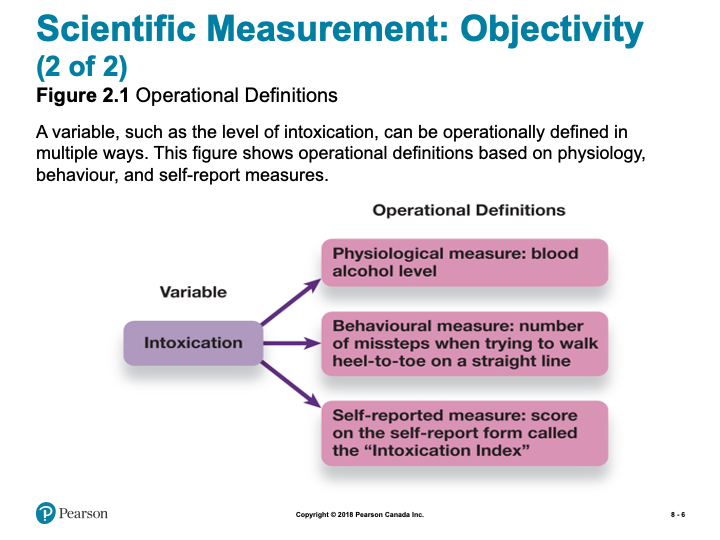
\includegraphics{assets/unit_1/PSYC106-Chs2-ResearchandThoughtandLanguage-3rdEd.png}

\emph{slide showing Operational Definitions}

Scientific Measurement: Reliability and Validity

\begin{itemize}
\tightlist
\item
  Reliability (p.~32)

  \begin{itemize}
  \tightlist
  \item
    Consistent and stable\\
  \end{itemize}
\item
  Validity (p.~32)

  \begin{itemize}
  \tightlist
  \item
    True measurements
  \end{itemize}
\end{itemize}

Generalizability of Results (1 of 2)

\begin{itemize}
\tightlist
\item
  Generalizability (p.~33)

  \begin{itemize}
  \tightlist
  \item
    Outside the laboratory\\
  \end{itemize}
\item
  Study large groups

  \begin{itemize}
  \tightlist
  \item
    Population (p.~33)

    \begin{itemize}
    \tightlist
    \item
      Sample (p.~33)
    \end{itemize}
  \end{itemize}
\end{itemize}

Generalizability of Results (2 of 2)

\begin{itemize}
\tightlist
\item
  Best reflection of population

  \begin{itemize}
  \tightlist
  \item
    Random sample (p.~33)\\
  \end{itemize}
\item
  Settle for easier sample

  \begin{itemize}
  \tightlist
  \item
    Convenience sample (p.~33)\\
  \end{itemize}
\item
  Location of study

  \begin{itemize}
  \tightlist
  \item
    Laboratory research\\
  \item
    Naturalistic research\\
  \item
    Ecological validity (p.~33)
  \end{itemize}
\end{itemize}

Sources of Bias in Psychological

\begin{itemize}
\tightlist
\item
  Research\\
\item
  Researcher Bias\\
\item
  Subject/Participant Bias\\
\item
  Hawthorne effect (p.~35)\\
\item
  Social Desirability (p.~35)
\end{itemize}

Working the Scientific Literacy Model: Demand Characteristics and
Participant Behaviour (1 of 2)

\begin{itemize}
\tightlist
\item
  What do we know about how bias affects research participants?

  \begin{itemize}
  \tightlist
  \item
    Demand characteristics (p.~36)\\
  \end{itemize}
\item
  How can science test the effects of demand characteristics on behaviour?

  \begin{itemize}
  \tightlist
  \item
    Backpack scenario
  \end{itemize}
\end{itemize}

Working the Scientific Literacy Model: Demand Characteristics and Participant Behaviour (2 of 2)

\begin{itemize}
\tightlist
\item
  How can we critically evaluate the issue of bias in research?

  \begin{itemize}
  \tightlist
  \item
    Researcher bias

    \begin{itemize}
    \tightlist
    \item
      Bright rats vs.~dull rats\\
    \end{itemize}
  \end{itemize}
\item
  Why is this relevant?

  \begin{itemize}
  \tightlist
  \item
    Bias compromises studies\\
  \item
    Placebo effect (p.~35)
  \end{itemize}
\end{itemize}

Psych @ The Hospital: The Placebo Effect

\begin{itemize}
\tightlist
\item
  Debate about placebo effect

  \begin{itemize}
  \tightlist
  \item
    ``All in their head''\\
  \item
    Actual physiological response\\
  \end{itemize}
\item
  Brain activity in regions involved in pain

  \begin{itemize}
  \tightlist
  \item
    Multiple ways for placebos to affect our responses to pain
  \end{itemize}
\end{itemize}

Techniques That Reduce Bias

\begin{itemize}
\tightlist
\item
  Anonymity\\
\item
  Confidentiality\\
\item
  Inform participants\\
\item
  Single-blind study (p.~37)\\
\item
  Double-blind study (p.~37)
\end{itemize}

Sharing the Results

\begin{itemize}
\tightlist
\item
  Academic journals

  \begin{itemize}
  \tightlist
  \item
    Peer review (p.~37)\\
  \item
    Replication (p.~38)
  \end{itemize}
\end{itemize}

Five Characteristics of Poor Research (1 of 2)

\begin{itemize}
\tightlist
\item
  Lack of falsifiable hypotheses (p.~38)

  \begin{itemize}
  \tightlist
  \item
    Testability requires faisifiability\\
  \end{itemize}
\item
  Anecdotal evidence (p.~38)

  \begin{itemize}
  \tightlist
  \item
    weight loss commercials\\
  \end{itemize}
\item
  Biased selection of data
\end{itemize}

Five Characteristics of Poor Research (2 of 2)

\begin{itemize}
\tightlist
\item
  Appeal to authority (p.~39)

  \begin{itemize}
  \tightlist
  \item
    Corresponding data?\\
  \item
    Biased expert?\\
  \end{itemize}
\item
  Appeal to common sense (p.~39)

  \begin{itemize}
  \tightlist
  \item
    Earth is centre of universe
  \end{itemize}
\end{itemize}

2.2 Learning Objectives

\begin{itemize}
\tightlist
\item
  Know the key terminology related to research designs.\\
\item
  Understand what it means when variables are positively or negatively correlated.\\
\item
  Understand how experiments help demonstrate cause-and-effect relationships.\\
\item
  Apply the terms and concepts of experimental methods to research examples.\\
\item
  Analyze the pros and cons of descriptive, correlational, and experimental research designs.
\end{itemize}

Descriptive Research (1 of 2)

\begin{itemize}
\tightlist
\item
  Descriptive data

  \begin{itemize}
  \tightlist
  \item
    From observations\\
  \item
    No attempt to explain why\\
  \end{itemize}
\item
  Qualitative Research (p.~42)
\end{itemize}

Descriptive Research (2 of 2)

\begin{itemize}
\tightlist
\item
  Case study (p.~42)

  \begin{itemize}
  \tightlist
  \item
    Extensive details\\
  \item
    Lacks generalizability\\
  \end{itemize}
\item
  Naturalistic observation (p.~44)
\item
  Self-reporting (p.~45)

  \begin{itemize}
  \tightlist
  \item
    Participant makes the observations
  \end{itemize}
\end{itemize}

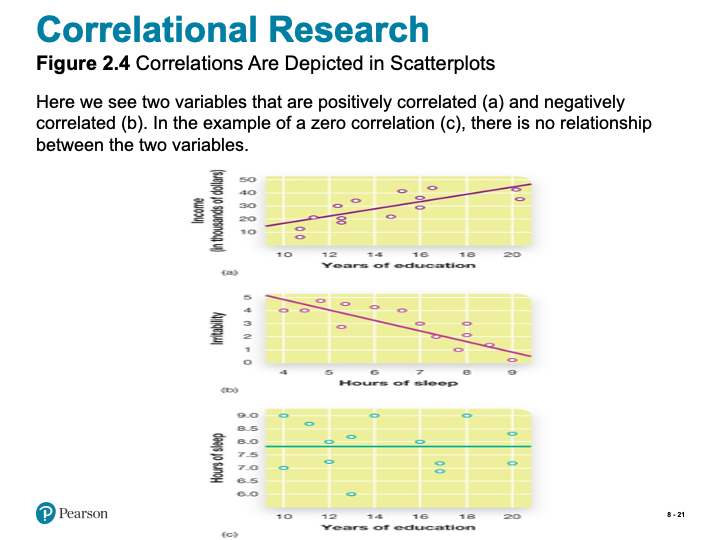
\includegraphics{assets/unit_1/slide_21.png}

\emph{Slide showing correlations depicted in scatterplots}

Myths in Mind: Beware of Illusory Correlations

\begin{itemize}
\tightlist
\item
  Illusory correlations (p.~47)

  \begin{itemize}
  \tightlist
  \item
    Crime increases when the moon is full
  \item
    Opposites attract
  \item
    Gamblers on a ``hot streak''
  \item
    Stereotypes
  \end{itemize}
\end{itemize}

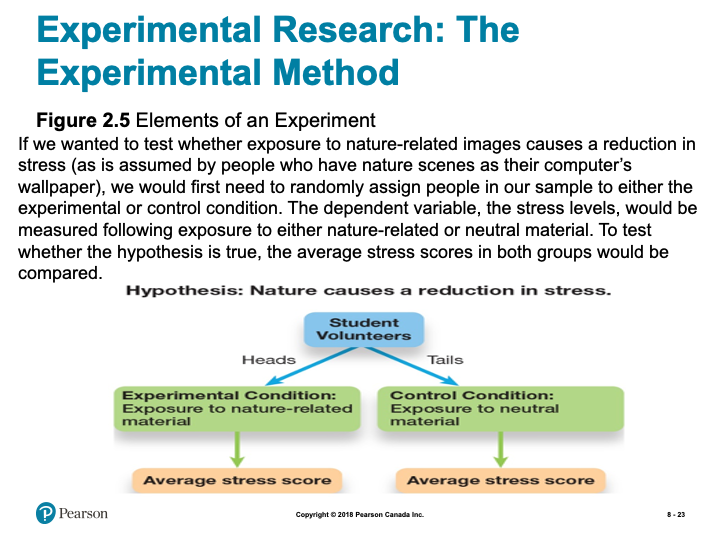
\includegraphics{assets/unit_1/slide_23.png}

\emph{Slide showing - Elements of an Experiment}

Experimental Research: The Quasi-Experimental Method

\begin{itemize}
\tightlist
\item
  Quasi-experimental research (p.~49)

  \begin{itemize}
  \tightlist
  \item
    Random assignment not always possible

    \begin{itemize}
    \tightlist
    \item
      Comparing men and women
    \end{itemize}
  \item
    Cannot determine cause-and-effect
  \end{itemize}
\end{itemize}

2.4 Learning Objectives

\begin{itemize}
\tightlist
\item
  Know the key terminology of statistics.\\
\item
  Understand how and why psychologists use significance tests.
\item
  Apply your knowledge to interpret the most frequently used types of graphs.
\item
  Analyze the choice of central tendency statistics based on the shape of the distribution.
\end{itemize}

Descriptive Statistics

\begin{itemize}
\tightlist
\item
  Descriptive statistics (p.~60)

  \begin{itemize}
  \tightlist
  \item
    Frequency
  \item
    Central tendency
  \item
    Variability
  \end{itemize}
\end{itemize}

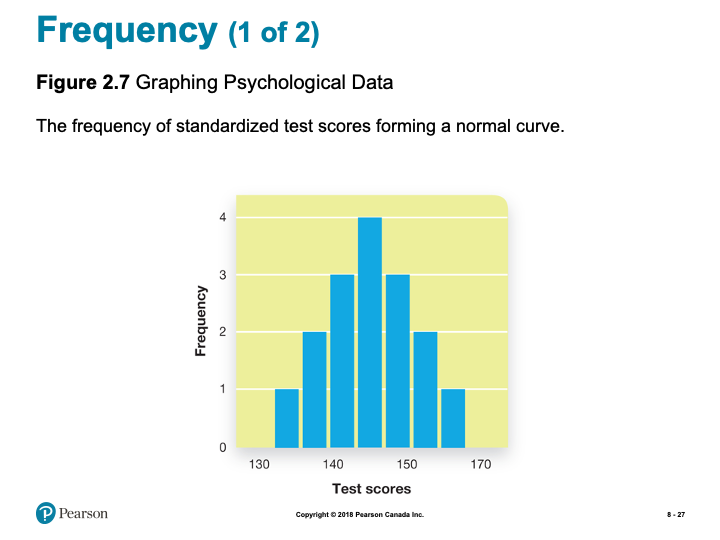
\includegraphics{assets/unit_1/slide_27.png}

\emph{Slide showing - Graphing Psychological Data}

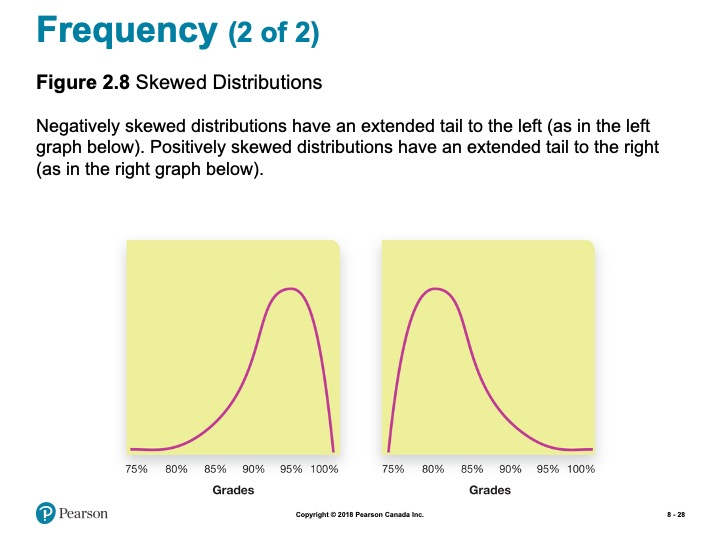
\includegraphics{assets/unit_1/slide_28.jpg}

\emph{Slide showing - Skewed Distributions}

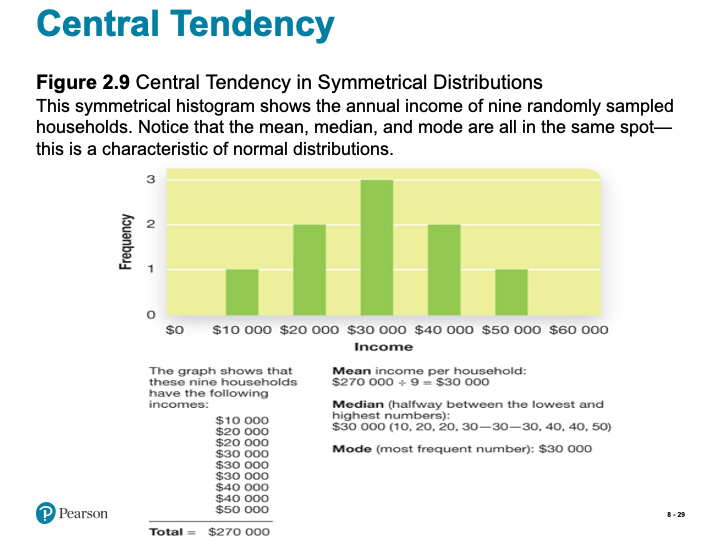
\includegraphics{assets/unit_1/slide_29.png}

\emph{Slide showing - Central Tendency in Symmetrical Distributions}

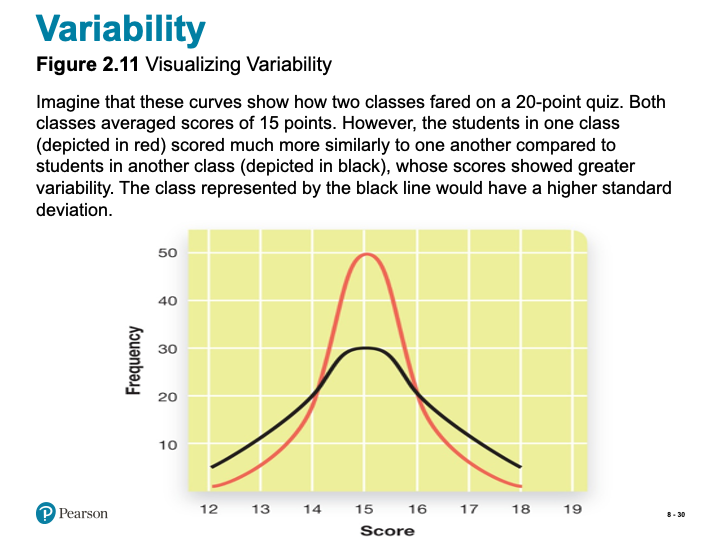
\includegraphics{assets/unit_1/slide_30.png}

\emph{Slide showing - Visualizing Variability}

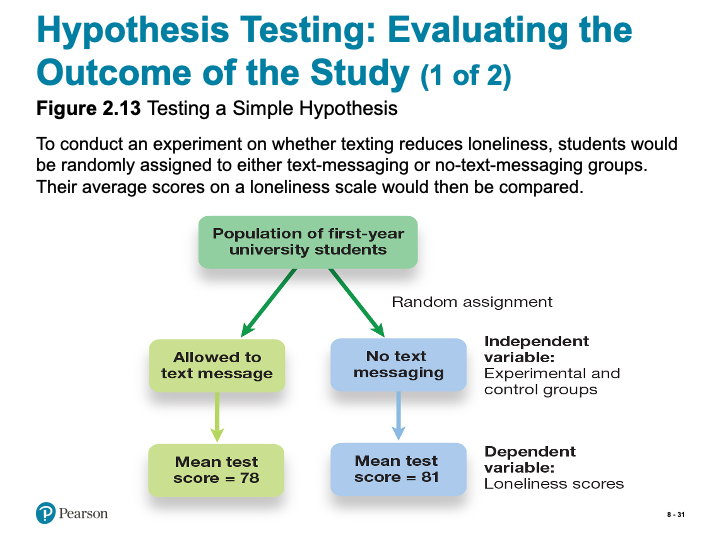
\includegraphics{assets/unit_1/slide_31.png}

\emph{Slide showing - Testing a Simple Hypothesis}

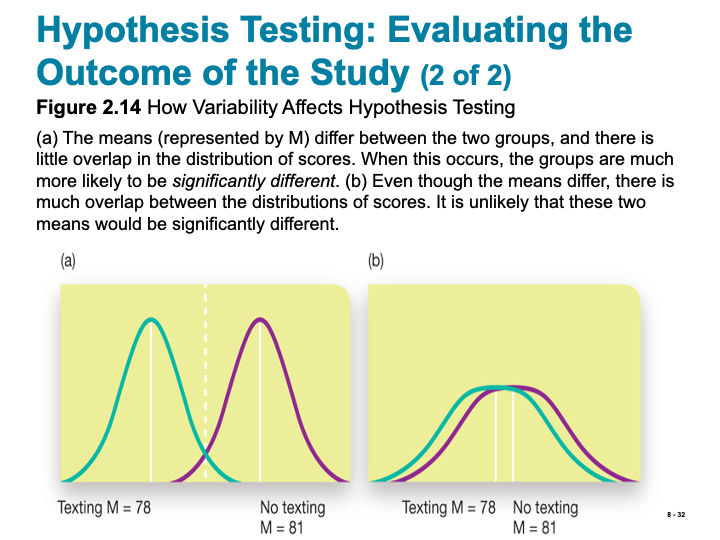
\includegraphics{assets/unit_1/slide_32.png}

\emph{Slide showing - How Variability Affects Hypothesis Testing}

True or False?

\begin{itemize}
\tightlist
\item
  T F 1. People more easily detect male prejudice against females than female against males or female against females.
\item
  T F 2. In general, people underestimate how much they really know.
\item
  T F 3. It takes less compelling evidence to change our beliefs than it did to create them in the first place.
\item
  T F 4. The babbling of an infant at 4 months of age makes it clear whether the infant is French, Korean, or Ethiopian.
\item
  T F 5. Some people can write but not read.
\item
  T F 6. Many bilinguals report that they have different senses of self, depending on which language they are using.
\item
  T F 7. Imagining a physical activity triggers action in the same brain areas that are triggered when actually performing that activity.
\item
  T F 8. Only human beings seem capable of insight (the sudden realization of a problem's solution).
\item
  T F 9. Honeybees do a dance to communicate the direction and distance of a new food source to other bees.
\item
  T F 10. Apes are capable of communicating meaning by using symbols.
\end{itemize}

Thinking

\begin{itemize}
\item
  Thinking, or cognition, refers to a process that involves knowing, understanding, remembering, and communicating.
\item
  Gr. {pove∞ - need to get the right characters for this word} (pr. phrones) - to think, to mind; to be of opinion; to take thought, be considerate; to entertain sentiments or inclinations of a specific kind, to be minded; to be in a certain frame of mind; to imagine; to heed, pay regard to; to incline to; be set upon, mind
\end{itemize}

A little more Greek

\begin{itemize}
\tightlist
\item
  Mind (Gr. { Noos- need to get the right characters for this word}) - the mind, intellect; understanding, intelligent faculty; intellect, judgment; opinion, sentiment; mind, thought, conception; settled state of mind; frame of mind.
\end{itemize}

The limits of intuition

\begin{itemize}
\tightlist
\item
  A bat and a ball cost \$1.10 in total. The bat costs \$1 more than the ball. How much does the ball cost?
\item
  A man bought a horse for \$60 and sold it for \$70. Then he bought the same horse back for \$80 and again sold it, for \$90. How much money did he make in the horse business?
\end{itemize}

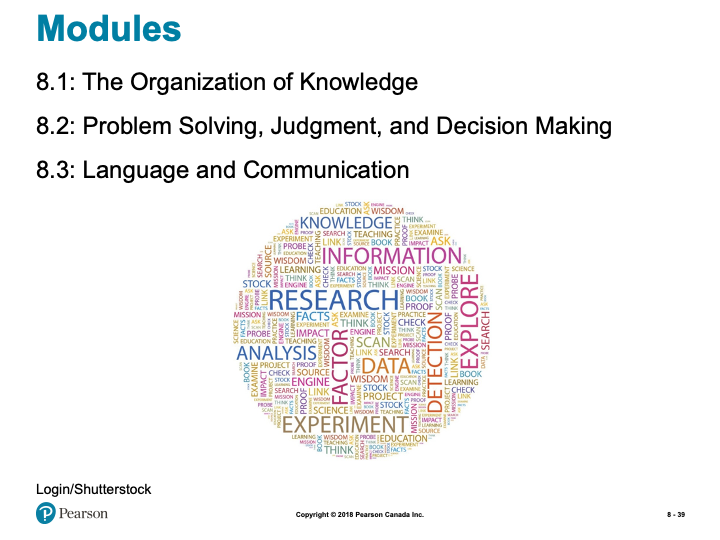
\includegraphics{assets/unit_1/slide_39.png}

\emph{Slide showing - Modules}

8.1 Learning Objectives

\begin{itemize}
\tightlist
\item
  Know the key terminology associated with concepts and categories.
\item
  Understand theories of how people organize their knowledge about the world.
\item
  Understand how experience and culture can shape the way we organize our knowledge.
\item
  Apply your knowledge to identify prototypical examples.
\item
  Analyze the claim that the language we speak determines how we think.
\end{itemize}

Concepts and Categories

\begin{itemize}
\tightlist
\item
  Concept (p.~294)

  \begin{itemize}
  \tightlist
  \item
    Divided into smaller groups
  \end{itemize}
\item
  Categories (p.~294)
\end{itemize}

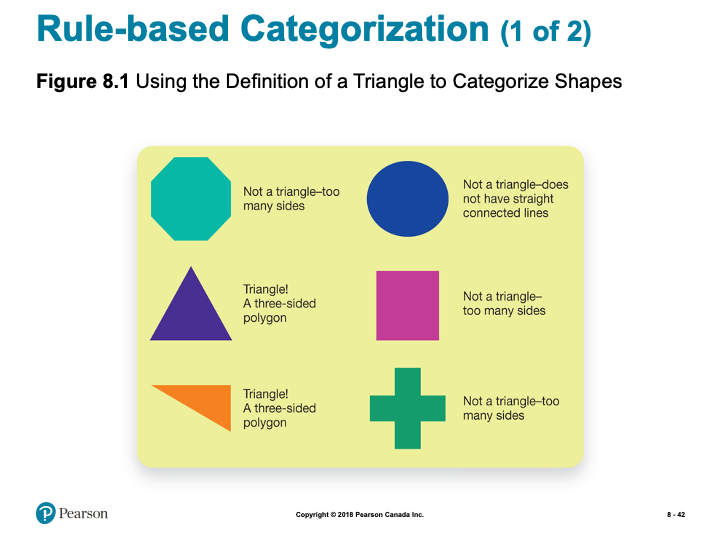
\includegraphics{assets/unit_1/slide_42.png}

\emph{Slide showing - Using the Definition of a Triangle to Categorize Shapes}

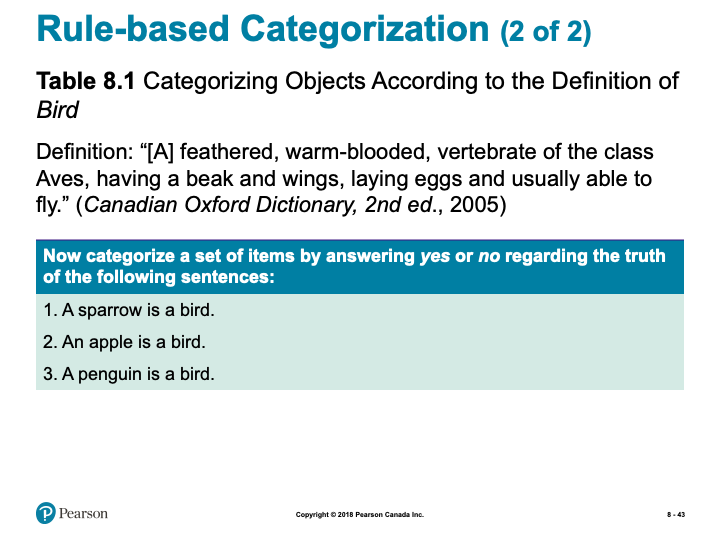
\includegraphics{assets/unit_1/slide_43.png}

\emph{Slide showing - Categorizing Objects According to the Definition of Bird}

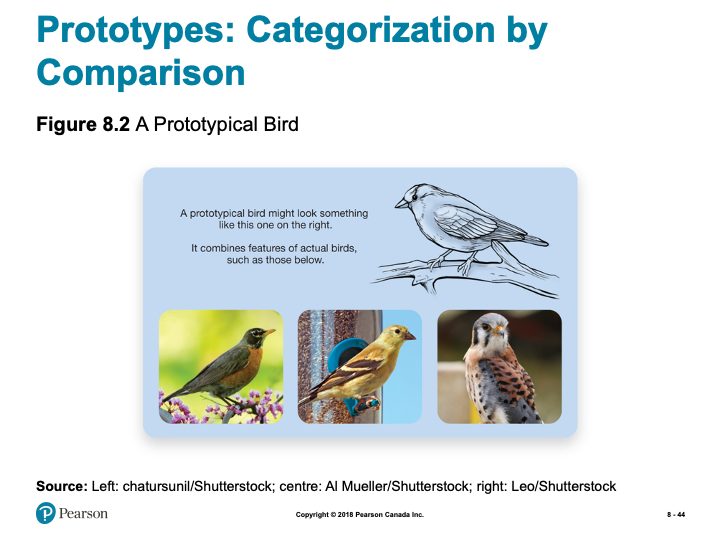
\includegraphics{assets/unit_1/slide_44.png}

\emph{Slide showing - A Prototypical Bird}

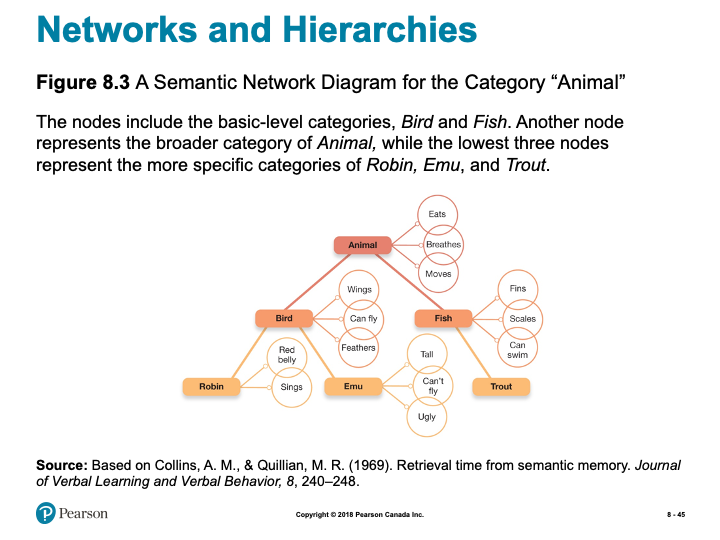
\includegraphics{assets/unit_1/slide_45.png}

\emph{Slide showing - A Semantic Network Diagram for the Category ``Animal''}

Working the Scientific Literacy Model: Priming and Semantic
Networks (1 of 2)

\begin{itemize}
\tightlist
\item
  What do we know about semantic networks?

  \begin{itemize}
  \tightlist
  \item
    Priming (p.~297)
  \end{itemize}
\item
  How can scientists explain priming effects?

  \begin{itemize}
  \tightlist
  \item
    Lexical Decision Task
  \end{itemize}
\end{itemize}

Working the Scientific Literacy Model: Priming and Semantic
Networks (2 of 2)

\begin{itemize}
\tightlist
\item
  Can we critically evaluate this information?

  \begin{itemize}
  \tightlist
  \item
    Strength of priming varies
  \item
    Experiments difficult to replicate
  \end{itemize}
\item
  Why is this relevant?

  \begin{itemize}
  \tightlist
  \item
    Advertising
  \end{itemize}
\end{itemize}

Categorization and Experience

\begin{itemize}
\tightlist
\item
  Categorization is based on experience

  \begin{itemize}
  \tightlist
  \item
    Efficient process
  \item
    But can also result in errors
  \end{itemize}
\end{itemize}

Categories and the Brain (1 of 2)

\begin{itemize}
\tightlist
\item
  Categories, Memories, and the Brain
\item
  Category-specific visual agnosia (CSVA)

  \begin{itemize}
  \tightlist
  \item
    Living vs.~non-living categories
  \end{itemize}
\end{itemize}

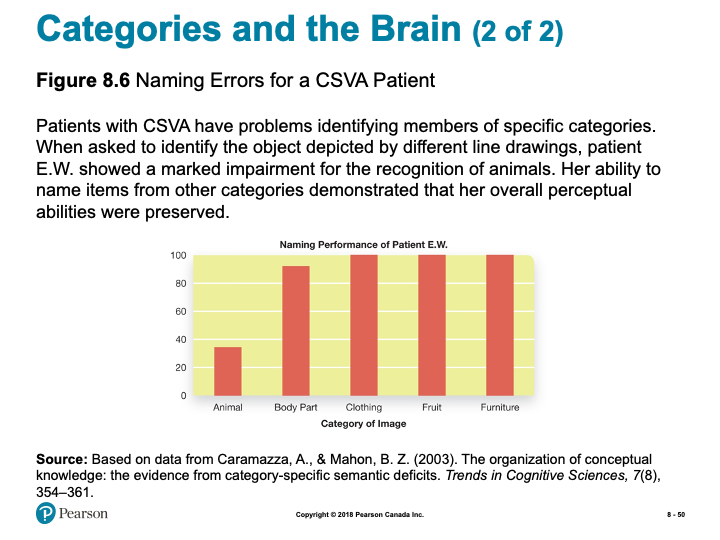
\includegraphics{assets/unit_1/slide_50.png}

\emph{Slide showing - Naming Errors for a CSVA Patient}

\begin{caution}
\textbf{Note:} the slides are intended to supplement the information found in your textbook. If you are having trouble viewing them, they can also be downloaded by scrolling to the bottom of the screen and clicking on the ``Unit 1- Slides'' link.*
\end{caution}

\hypertarget{learning-activities}{%
\subsection*{Learning Activities:}\label{learning-activities}}
\addcontentsline{toc}{subsection}{Learning Activities:}

\begin{reflect}
\textbf{Chapter 2 Review Quiz}

\begin{itemize}
\tightlist
\item
  Practice Quiz to self-assess your own comprehension of important terms from Chapter 2.\\
\item
  Not for formal evaluation.
\end{itemize}

\textbf{Problem Solving Activity}

\begin{itemize}
\tightlist
\item
  Solve some problems by utilizing some of the cognitive strategies we learned about in this topic.
\end{itemize}

\textbf{Problem Solving Practice}

\begin{itemize}
\tightlist
\item
  Explore problem solving activities and reflect on the strategies you incorporate as you discover solutions.
\end{itemize}

\textbf{Introduction to Visualization}

\begin{itemize}
\tightlist
\item
  Article introduces visualization and provides an opportunity to practice this skill.
\end{itemize}

\textbf{Learning Lab Preparation}

\begin{itemize}
\tightlist
\item
  Each topic will provide a question or scenario for you to consider prior to attending your Learning Lab. Be sure to carefully consider each prompt as you will be expected to contribute to the group discussion.
\end{itemize}
\end{reflect}

\hypertarget{resources}{%
\subsection*{Resources}\label{resources}}
\addcontentsline{toc}{subsection}{Resources}

Here are some additional resources that will help you complete this unit:

\begin{itemize}
\tightlist
\item
  Krause, M., Corts, D., Smith, S. C., \& Dolderman, D. (2018). \emph{Revel for An Introduction to Psychological Science, 2nd Canadian Edition.} Pearson Ed.\\
\item
  Other resources will be provided online.
\end{itemize}

\hypertarget{what-is-psychology}{%
\section{What is Psychology}\label{what-is-psychology}}

We begin our course with a quick challenge: \textbf{\emph{In your own words, define ``psychology.''}}

According to your definition, how is psychology different from other academic areas that would study humans (\emph{for example, philosophy, literature, or history})? If you said ``Pyschology is different because it uses the scientific method''- give yourself a pat on the back

You will begin your study of the scientific method by reading your textbook. The parable below (\emph{from Philipchalk's Social Psychology textbook}), however, helps illustrate the scientific method with three ``helpful'' approaches to a problem, including a simple experiment:

\emph{Once upon a time there were three brothers. One day while they were working in their father's field, they saw an old man coming along the road. The old man greeted them, and then struggled on along the road, limping terribly. After that, every day at the same time, the brothers greeted the old man and watched as he hobbled by. When a month had passed, they were so impressed that they each did something. The first brother wrote a compelling story about perseverance in the face of the ravages of old age. It encouraged many people. The second brother painted a moving portrait of the old man, stooped over and limping along. People were inspired. The third brother, who had observed the old man very closely, asked him one day if he could exchange shoes with him. The old man was surprised, but he gladly agreed. When the old man walked away he did not limp. The next day the third brother gave the old man his shoes back and watched as he limped on his way. On the third day, the brother again exchanged shoes with the old man. Then he took the old man's shoes to a shoemaker and had them repaired. When the brother gave them back to the old man he was delighted. The old man put on the shoes, thanked the brother, and walked away without a limp.}

Although each brother made a positive contribution, the third brother solved the man's problem because he discovered its cause. To do this, \textbf{\emph{he used the scientific method and he conducted an experiment (Philipchalk, 1994).}}

I think psychology is one of the most interesting areas of study there is, first, because it studies people, people like you and me, and we're interesting Second, I like psychology because it is so broad. Psychologists, as you will soon see, study everything from nerve conduction in single cells, all the way to the influence of groups on our behaviour---and everything in between. Finally, psychologists don't just speculate and theorize, they look for evidence for their ideas. If they don't find sufficient evidence, they change their ideas; and I like that. Which leads us back to the scientific method and how psychology began.

\hypertarget{learning-activity}{%
\subsection*{Learning Activity}\label{learning-activity}}
\addcontentsline{toc}{subsection}{Learning Activity}

\begin{reflect}
\textbf{Chapter 2 Review Quiz}

In order to review some of the major concepts from the text, take the following unmarked quiz. Although you will not be evaluated on these terms, they will assist you in the assignments for this course.
\end{reflect}

\hypertarget{thinking-and-problem-solving}{%
\section{Thinking and Problem Solving}\label{thinking-and-problem-solving}}

\hypertarget{thinking}{%
\subsection*{Thinking}\label{thinking}}
\addcontentsline{toc}{subsection}{Thinking}

``So God created man in his own image, in the image of God created he him; male and female created he them.'' (Genesis 1:27)

``I will praise thee; for I am fearfully and wonderfully made.'' (Psalm 139:14)

The human image of God means many things. It seems that one aspect of this image is our thinking ability, including our ability to solve problems and speak. How important is our thinking ability in our reflection of God's image? What does your answer mean for people with less ability? What about people who lose abilities due to accident or disease (e.g., Alzheimer's patients)?

\hypertarget{algorithms-heuristics}{%
\subsection*{Algorithms \& Heuristics}\label{algorithms-heuristics}}
\addcontentsline{toc}{subsection}{Algorithms \& Heuristics}

Algorithms and heuristics can be confusing. An algorithm is a guaranteed route to a solution, but it may be the long way around to success. If you knew a person lived somewhere in a large residence hall, an algorithm for finding that individual would be to knock on every door until you located the person. Heuristics, on the other hand, sug­gest that you would first ask friends where to locate the person, or check a list, then knock on the appropriate door to locate the person. Another way to think of heuristics is the phrase ``rule of thumb.'' Can you think of some rules of thumb that you have learned from your various job experiences? They may have to do with how long to cook a hamburger, or when to refill a machine, or how to get a date.

Consider the following example and explanation taken from Invitation to Social Psychology by Ron Philipchalk:

\emph{In the second part of the book, they tell you how to crack a safe. There are all kinds of ninny-pinny, dopey things, like ``It might be a good idea to try a date for the combination, because lots of people like to use dates.'' Or ``Think of the psychology of the owner of the safe, and what he might use for the combination.'' And ``The secretary is often worried that she might forget the combination of the safe, so she might write it down in one of the following places---along the edge of her desk drawer, on a list of names and addresses . . .'' and so on . . . .}

\emph{I also did a certain amount of systematic study. For instance, a typical combination was 69-32-21. How far off could a number be when you're opening the safe? If the number was 69, would 68 work? Would 67 work? On the particular locks we had, the answer was yes for both, but 66 wouldn't work. You could be off by two in either direction. That meant you only had to try one out of five numbers, so you could try zero, five, ten, fifteen, and so on. With twenty such numbers on a wheel of 100, that was 8000 possibilities instead of the 1,000,000 you would get if you had to try every single number. . . .}

\emph{I practiced all the time on my own safe so I could do this process as fast as I could and not get lost in my mind as to which number I was pushing and mess up the first number. Like a guy who practices sleight of hand, I got it down to an absolute rhythm so I could try the 400 possible back numbers in less than half an hour. That meant I could open a safe in a maximum of eight hours---with an average time of four hours. (Surely You're Joking Mr.~Feynman, p.~140)}

Mr.~Feynman's safecracking system succeeds because he methodically works through every possible combination. By logical analysis he has discovered which 8,000 possibilities out of 1,000,000 he needs to try. We call this type of logical step-by-step procedure for solving problems an algorithm (Newell \& Simon, 1972; Simon, 1981). If you use the correct algorithm your success is guaranteed.

But sometimes it can take a long time to discover the correct algorithm. And employing an algorithm is often time consuming. Mr.~Feynman spent days developing his system and it took hours to open a safe. You could certainly open a safe much faster if you found the combination on the edge of the secretary's drawer.

The shortcuts Mr.~Feynman calls ``ninny-pinny, dopey things'' are examples of heuristics. Heuristics are rule-of-thumb strategies for solving problems, shortcuts we develop from our experience. Heuristics often help us eliminate improbable alternatives and guide us to the most likely solution to a problem. Despite his appreciation for algorithms, Mr.~Feynman discovered heuristics can be useful. He found, for example, that safe owners often did not bother to change the factory set combination when they received a new safe. In one office building the temporary factory combinations 25-0-25 or 50-25-50 opened one safe in five

Algorithms and heuristics are examples of cognitive strategies---mental plans we use to make decisions and solve problems.

\hypertarget{learning-activities-1}{%
\subsection*{Learning Activities}\label{learning-activities-1}}
\addcontentsline{toc}{subsection}{Learning Activities}

\textbf{Read and Reflect}

In addition to the content above, you are also responsible for reading through the following:

\emph{Krause et. al (2018). Revel for An Introduction to Psychological Science, 2nd Canadian Edition. Chapter 8}

While all of these pages may not relate directly to this unit's discussion, consistent reading will help you keep pace, as well as provide necessary background knowledge when you need it.

\textbf{Problem Solving Activity}

In this lesson, we spent time exploring cognitive strategies used to solve problems and make decisions. We now have an opportunity to practice this on our own Take a look at the following problems and see if you can find a solution. As you work through the problems, think about what cognitive strategies you are implementing as you make each decision:

\textbf{\emph{Problem A}}

\begin{itemize}
\tightlist
\item
  Take a look at the following Roman Numeral: \textbf{IX}
\item
  Now add one line to the Roman numeral \textbf{IX} to make it six
\end{itemize}

Click here for the solution.

\begin{verbatim}
The answer is to add a curved line shaped like an "S" (i.e., "SIX"). In writing, the problem looks simple, but you might want to try it aloud on a friend. There is a mental set that one must add a straight line and have some form of Roman numeral on the page.
\end{verbatim}

\textbf{\emph{Problem B}}

Your task is to plant trees on Arbor Day. You have ten trees that must be planted in five rows of four trees each. How would you plant the trees?

Click here for the solution.

The answer is that you would arrange them at the vertices and cross-points of a 5-pointed star

\hypertarget{learning-activity-1}{%
\subsection*{Learning Activity :}\label{learning-activity-1}}
\addcontentsline{toc}{subsection}{Learning Activity :}

\textbf{Problem Solving Practice}

Below is a website that provides more opportunity to work through, and solve, some problems. Specifically, this resource explores the idea of \textbf{\emph{Assumptions}} and the role assumptions play when solving problems. Furthermore, this is a valuable resource as it also explores other important techniques to be implemented when solving problems.

Click on the following link and read through the information as you continue to practice your problem solving:

\href{https://www.virtualsalt.com/crebook4.htm}{\textbf{Virtual Salt}}

\hypertarget{learning-lab-preparation}{%
\subsubsection*{Learning Lab Preparation}\label{learning-lab-preparation}}
\addcontentsline{toc}{subsubsection}{Learning Lab Preparation}

Your Learning Lab for this unit will focus on group discussion as explore the topics of this unit in more detail. As you prepare for your Learning Lab, one possible scenario that discussion will focus on is below- please prepare some thoughts to share with the group:

In the largest sense, society is breaking into two classes:

\emph{The first class are people who know how to think. These people realize that most problems are open to examination and creative solution. If a problem appears in the lives of these people, their intellectual training will quickly lead them to a solution or an alternative statement of the problem. These people are the source of the most important product in today's economy -- ideas.}

\emph{The second class, the vast majority of society, are people who cannot think for themselves. I call these people `idea consumers' -- metaphorically speaking, they wander around in a gigantic open-air mall of facts and ideas. The content of their experience is provided by television, the Internet and other shallow data pools. These people believe collecting images and facts makes them educated and competent, and all their experiences reinforce this belief. The central, organizing principle of this class is that ideas come from somewhere else, from magical persons, geniuses, `them.'}

Consider the following prompts to help better prepare for the discussion:

\begin{itemize}
\tightlist
\item
  \textbf{\emph{Do you agree or disagree with this claim?}}\\
\item
  \textbf{\emph{Do you know people that fit in the second category? What causes this difference? How might it be changed?}}
\end{itemize}

\hypertarget{cognitive-biases}{%
\section{Cognitive Biases}\label{cognitive-biases}}

As if the biases mentioned in the textbook are not enough, here are a few more to watch out for, taken from Invitation to Social Psychology by Ron Philipchalk.

\hypertarget{the-gamblers-fallacy}{%
\subsection*{The Gambler's Fallacy}\label{the-gamblers-fallacy}}
\addcontentsline{toc}{subsection}{The Gambler's Fallacy}

Jill and Bob are the parents of three boys. Jill is pregnant again, and she and Bob are hoping the baby is a girl. In fact, they are confident the baby must be a girl because their previous three children were boys. If you agree with Jill and Bob that the baby is more likely to be a girl than a boy, then you---along with Jill and Bob---may be committing the gambler's fallacy. No matter how many boys have been born, the likelihood of a girl being born is the same as it always was, approximately 50 \% (assuming no biological abnormality or medical intervention).

The gambler's fallacy arises from our failure to recognize the independence of unconnected events. The result of a coin toss does not depend on the outcome of previous tosses; a child's sex at conception is not affected by the sex of prior conceptions; the cards dealt in a hand are not influenced by the distribution of cards on the previous deal; and so on. Each event in these sequences is independent of the others, although we tend to think that somehow there must be a connection.

\hypertarget{the-anchoring-and-adjustment-heuristic}{%
\subsection*{The Anchoring and Adjustment Heuristic}\label{the-anchoring-and-adjustment-heuristic}}
\addcontentsline{toc}{subsection}{The Anchoring and Adjustment Heuristic}

First impressions of a person exert a powerful influence on the way we interpret subsequent information about that person. This effect may be an example of a more general principle called the anchoring and adjustment heuristic. Information we use to establish a starting value (or anchor point) tends to be more influential in our decisions than subsequent information we use to adjust this value (Tversky \& Kahneman, 1974).

Daniel Cervone and his colleagues found, for example, that initial success or failure on a task can establish an anchor for feelings of self-efficacy. Students who initially succeed on a task and later fail have higher feelings of self-efficacy than students who initially fail and later succeed even though their overall level of success is the same. Final judgments of self-efficacy are biased in the direction of initial judgments (Cervone \& Palmer, 1990; Peake \& Cervone, 1989).

Salespeople often use the anchoring and adjustment heuristic to their advantage. Some real estate agents routinely show their clients an over-priced and unattractive house first in order to set an anchor point which, in effect, says, ``The kind of house you want is going to cost a lot.'' Once established, this expectation of high price changes very slowly and the clients are relieved to find an acceptable house in their price range (Northcraft \& Neale, 1987).

Car dealers too like us to set our sights high. Their so-called list price establishes an anchor or reference point that overshadows our subsequent evaluations, as I recently discovered. In looking for a certain model of car, I was attracted to a particular vehicle with an asking price of \$3,800 (``reduced from \$4,200''). I believed this price was too high, so I bargained with the vendor. Eventually, I bought the car for \$2,800. Did the high original asking price affect my decision? Yes, it probably did. Subsequent events indicated I still paid too much. I later bought an identical model in only slightly poorer condition for \$2,000. I was a victim of the anchoring and adjustment heuristic.

\textbf{\emph{Contrast Effects}}

My car purchase also illustrates a related distortion in judgment, the contrast effect. In contrast to the original price of \$4,200 my offer of \$2,800 seemed like a bargain. John Lynch, Jr.~and his colleagues (1991) found a similar effect with students. The students rated low-priced cars as less expensive when they were considered alongside high-priced cars (contrast effect), compared to when they were considered along with other low-priced cars (no contrast).

Research by Douglass Kenrick and his colleagues indicates that we also show contrast effects in evaluating other people. In one study (1980), male college students rated the attractiveness of potential blind dates. Subjects who gave their ratings after watching a TV show with attractive female actresses rated the potential dates as less attractive than did subjects who rated their potential dates before watching the show. In another study (1989), after viewing centerfold erotica, men found average women---and even their own wives---less attractive.

\hypertarget{heuristics-biases}{%
\subsection*{Heuristics \& Biases}\label{heuristics-biases}}
\addcontentsline{toc}{subsection}{Heuristics \& Biases}

By now you may be wondering why we fall prey to so many cognitive biases and errors. Well don't worry; our biases are actually a side effect of our cognitive efficiency. Most of our biases result from using heuristics, rules of thumb, or mental shortcuts that work very well. Sometimes they let us down, but overall, they improve the speed with which we handle mental problems---much like Mr.~Feynman's safe-cracking tricks. As we noted in the previous discussion, you could certainly open a safe much faster if you found the combination on the edge of the secretary's drawer. However, you won't always find the combination there, so limiting yourself to this approach would produce a kind of ``cognitive bias'' in your safe-cracking strategy.

\hypertarget{resources-online-articles-of-interest}{%
\subsection*{RESOURCES: Online Articles of Interest}\label{resources-online-articles-of-interest}}
\addcontentsline{toc}{subsection}{RESOURCES: Online Articles of Interest}

For additional information and examples, click on the link below:

\href{https://en.wikipedia.org/wiki/List_of_cognitive_biases}{\textbf{Cognitive Biases}}

\hypertarget{learning-lab-preparation-1}{%
\subsection*{Learning Lab Preparation}\label{learning-lab-preparation-1}}
\addcontentsline{toc}{subsection}{Learning Lab Preparation}

Another focus of our discussion during our Learning Lab for this unit, will focus on biases. In order to prepare for participation in this discussion, consider the guiding prompt below- be sure to have some thoughts to contribute to the discussion:

\textbf{\emph{Give an example from your own experience of one of the cognitive biases, discussed here or in the textbook, that you have fallen prey to.}}

\hypertarget{language-and-thought}{%
\section{Language and Thought}\label{language-and-thought}}

\hypertarget{linguistic-relativity}{%
\subsection*{Linguistic Relativity}\label{linguistic-relativity}}
\addcontentsline{toc}{subsection}{Linguistic Relativity}

Benjamin Whorf's linguistic relativity hypothesis suggests that our language affects the way we see the world. Do you know any examples of weather terms, for example, that are unique to one area? Could knowing these terms help you to notice differences in weather that outsiders might not notice? What about in sports? Sports fans usually know terms to de­scribe certain strokes or plays. Does knowledge of these terms affect percep­tion? Can you think of some examples? What does it mean to ``clothesline'' someone, or ``post-up,'' or ``birdie?''

\hypertarget{imaginary-practice}{%
\subsection*{Imaginary Practice}\label{imaginary-practice}}
\addcontentsline{toc}{subsection}{Imaginary Practice}

Mental practice is now widely accepted in many areas. The following excerpt is taken from the \href{https://www.golfpsych.com}{\textbf{GolfPsych}} website. You may find further examples there as well.

``You can practice the mental aspects of your game anytime. We encourage our clients to do imagery practice of playing well in upcoming tournaments. This imaginary practice includes seeing the course, situation, doing a full mental pre-shot routine and seeing a good shot. You should also be feeling the way you do when you play your best. In addition, you should be practicing deep breathing and quieting your mind off-course. This is an extremely valuable tool that must be practiced to be effective. The mental game is much more than thinking positive thoughts. Take our Personality Assessment and get your own GolfPsych Report to receive our recommendations for you based on your personality and our research. Reading our book will also help you understand all aspects of a good mental game. During your practices and before your rounds you should also be practicing your mental skills.''

\hypertarget{learning-activity-2}{%
\subsection*{Learning Activity}\label{learning-activity-2}}
\addcontentsline{toc}{subsection}{Learning Activity}

\hypertarget{introduction-to-visualization}{%
\subsubsection*{Introduction to Visualization}\label{introduction-to-visualization}}
\addcontentsline{toc}{subsubsection}{Introduction to Visualization}

In this Topic, we learned about the notion of mental practice. Below is an article that will take you through the process of visualization. Take some time to read the article and practice for yourself. Pay careful attention to your thoughts, your focus, your feelings as you engage in the process.

\begin{itemize}
\tightlist
\item
  \href{https://www.forbes.com/sites/bhaligill/2017/06/22/new-to-visualization-here-are-5-steps-to-get-you-started/\#60dafcdc6e3f}{\textbf{Introduction to Visualization}}
\end{itemize}

\hypertarget{learning-lab-preparation-2}{%
\subsubsection*{Learning Lab Preparation}\label{learning-lab-preparation-2}}
\addcontentsline{toc}{subsubsection}{Learning Lab Preparation}

The subject of our focus for this Topic has been on the power of language in influencing how we see the world. Our discussion during Learning Lab this week will focus on the importance of language in the Bible (and other religious writings) and how it ``shapes'' how we see the world.

To prepare for this discussion, consider the following prompt:

\textbf{\emph{Give some examples of the importance of language in the Bible or other religious writings.}}

\hypertarget{animal-language}{%
\section{Animal Language}\label{animal-language}}

\hypertarget{language}{%
\subsection*{Language}\label{language}}
\addcontentsline{toc}{subsection}{Language}

As a Christian I am pleased to see in psychology the resurgence of interest in studying some of what Ronald Koteskey (1980) calls humanity's ``God-like'' characteristics, creativity, imagery, and particularly language.

The use of words is extremely important in Christian scripture. God spoke the creation into existence; Jesus is called the Word; the significance of Babel and Pentecost are closely linked to the importance of language; and there is great power associated with an individual's name. In addition, Christians have usually considered the ability to communicate with words to be part of the image of God in man. However, recently several researchers claim to have taught animals, usually chimpanzees or apes, to communicate through language. Using sign language, blocks, or keyboards and computer- generated voices, the animals have signaled their needs and even generated word combinations.

But is this truly language? There is no doubt that the animals are using symbols as signs to stand for objects and actions. However, there are significant questions being raised about the comparison with human language.

Christians need to think carefully about what they mean when they talk about the image of God in man. The area of human learning and psycholinguistics offers some intriguing questions for thoughtful Christians. What is the origin of human speech-is it learned (as Skinner would say) or largely innate (as Chomsky would say)? Is human speech unique? Do the studies of language in animals necessitate a redefinition of the uniqueness of man? (Based on Psychology and Christianity by Ron Philipchalk, p.~102)

\hypertarget{resources-online-articles-of-interest-1}{%
\subsubsection*{RESOURCES: Online Articles of Interest}\label{resources-online-articles-of-interest-1}}
\addcontentsline{toc}{subsubsection}{RESOURCES: Online Articles of Interest}

To add to our exploration of this topic, take a moment to read the following articles:

\begin{itemize}
\item
  \href{http://tuvalu.santafe.edu/~johnson/articles.chimp.html}{\textbf{Chimp Talk Debate: Is It Really Language?}}
\item
  \href{https://www.massey.ac.nz/~alock/hbook/ristau.htm}{\textbf{Animal Language and Cognition Projects}}
\end{itemize}

\hypertarget{learning-lab-preparation-3}{%
\subsubsection*{Learning Lab Preparation}\label{learning-lab-preparation-3}}
\addcontentsline{toc}{subsubsection}{Learning Lab Preparation}

Finally, take a moment to consider the following questions:

\textbf{\emph{How important for our understanding of who we are as humans is the distinctiveness of our language ability? Is it a sign of the image of God?}}

Be prepared to share your thoughts during discussion at your Learning Lab.

\hypertarget{assessment}{%
\section*{Assessment}\label{assessment}}
\addcontentsline{toc}{section}{Assessment}

While there is no ``formal'' assignment that you will be responsible for submitting for Unit 1, you will be expected to participate in discussion during your Learning Lab. Your facilitator will be providing a participation mark based on your contributions. Below is some information to consider prior to attending your Learning Lab:

\emph{Active participation in group exercises, reflection, and critical discourse is an essential component of this course. You are expected to show respect for all members of the course, both in your speech and actions. Contribute by actively observing and listening, raising thoughtful questions, examining relevant issues, building on others' ideas, analyzing and evaluating the group's thinking, synthesizing key points, and expanding the group's perspectives. Take care not to dominate a conversation, giving space for others to speak. When in small groups help maintain the focus, flow, and quality of conversations, and take the initiative to invite others (particularly those who are quiet) to speak.}

\textbf{Rubric for Participation in Learning Labs}

\begin{longtable}[]{@{}
  >{\raggedright\arraybackslash}p{(\columnwidth - 4\tabcolsep) * \real{0.3333}}
  >{\raggedright\arraybackslash}p{(\columnwidth - 4\tabcolsep) * \real{0.3333}}
  >{\raggedright\arraybackslash}p{(\columnwidth - 4\tabcolsep) * \real{0.3333}}@{}}
\toprule\noalign{}
\begin{minipage}[b]{\linewidth}\raggedright
Emerging (0-64\%)
\end{minipage} & \begin{minipage}[b]{\linewidth}\raggedright
Developing (65-89\%)
\end{minipage} & \begin{minipage}[b]{\linewidth}\raggedright
Mastering (90-100\%)
\end{minipage} \\
\midrule\noalign{}
\endhead
\bottomrule\noalign{}
\endlastfoot
Never to almost never: Demonstrates active listening (as indicated by disengaged body language and no to rare comments that build on others' remarks),Initiates any contributions in class or small groups, Makes insightful or constructive comments, Helps maintain a supportive space for others to speak. & Sometimes to fairly often: Demonstrates active listening (as indicated by somewhat to often engaged body language and comments that build on others' remarks), Initiates a contribution at least once in a class or small group discussion; Makes insightful or constructive comments, Helps maintain a supportive space for others to speak. & Very often to nearly always: Demonstrates active listening (as indicated by fully engaged body language and comments that build on others' remarks), Initiates more than one contribution in a class or small group discussion, Makes insightful or constructive comments, Creates a space for others to speak and takes initiative to include others. \\
\end{longtable}

\hypertarget{checking-your-learning}{%
\section*{Checking your Learning}\label{checking-your-learning}}
\addcontentsline{toc}{section}{Checking your Learning}

Before you move on to the next unit, check that you are able to:

\begin{itemize}
\tightlist
\item
  Define key terminology related to principles of scientific research, research designs, and statistics.
\item
  Explain the five characteristics of quality scientific research, and the pros and cons of descriptive, correlational, and experimental research designs.
\item
  Determine how biases might influence the outcome of a study and how experiments help demonstrate cause-and-effect relationships.
\item
  Apply the concepts of reliability and validity to examples and concepts of experimental methods to research examples.
\item
  Assess whether anecdotes, authority figures, and common sense are reliably truthful sources of information.
\item
  Understand what it means for variables to be positively or negatively correlated and how and why psychologists use significance tests.
\end{itemize}

\hypertarget{title}{%
\chapter{Title}\label{title}}

\hypertarget{title-1}{%
\chapter{Title}\label{title-1}}

\hypertarget{title-2}{%
\chapter{Title}\label{title-2}}

\hypertarget{title-3}{%
\chapter{Title}\label{title-3}}

\hypertarget{title-4}{%
\chapter{Title}\label{title-4}}

\hypertarget{sample-unit-format}{%
\chapter*{Sample Unit Format}\label{sample-unit-format}}
\addcontentsline{toc}{chapter}{Sample Unit Format}

\hypertarget{overview-1}{%
\section*{Overview}\label{overview-1}}
\addcontentsline{toc}{section}{Overview}

In this first unit, we begin the course by\ldots{}

\hypertarget{topics-1}{%
\section*{Topics}\label{topics-1}}
\addcontentsline{toc}{section}{Topics}

\begin{enumerate}
\def\labelenumi{\arabic{enumi}.}
\tightlist
\item
  \emph{Topic}\\
\item
  \emph{Topic}\\
\item
  \emph{Topic}\\
\item
  \emph{Topic}
\end{enumerate}

\hypertarget{learning-outcomes-1}{%
\section*{Learning Outcomes}\label{learning-outcomes-1}}
\addcontentsline{toc}{section}{Learning Outcomes}

\begin{itemize}
\tightlist
\item
  \emph{Describe\ldots{}}
\item
  \emph{Contrast\ldots{}}
\item
  \emph{Analyze\ldots{}}
\item
  \emph{Determine\ldots{}}
\item
  \emph{Create\ldots{}}
\end{itemize}

\hypertarget{activity-checklist-1}{%
\section*{Activity Checklist}\label{activity-checklist-1}}
\addcontentsline{toc}{section}{Activity Checklist}

Here is a checklist of learning activities you will benefit from in completing this unit. You may find it useful for planning your work.

\begin{reflect}
{Unit 1 Learning Activities }

\begin{itemize}
\tightlist
\item
\item
\end{itemize}
\end{reflect}

\begin{assessment}
{Unit 1 Assessment}

Please check Moodle for details on what you are required to present for this unit.
\end{assessment}

\begin{feedback}
\textbf{Tips for Instructors:}
Learning activities are typically ungraded, and can be optional for students, however they are designed to help students learn the material and prepare for the assignments.
\end{feedback}

\hypertarget{resources-1}{%
\section*{Resources}\label{resources-1}}
\addcontentsline{toc}{section}{Resources}

Here are the resources you will need to complete this unit.

\begin{itemize}
\tightlist
\item
\item
\end{itemize}

\hypertarget{topic-1-title}{%
\section{Topic 1 Title}\label{topic-1-title}}

{[}Add content{]}

\begin{feedback}
\textbf{Tips for Instructors:} Topic content can be 1-2 paragraphs or several pages. Consider using instructional videos, graphics, charts, or other images to convey information and appeal to visual learners.
\end{feedback}

\hypertarget{activity-introductory-readings-video}{%
\subsection*{Activity: Introductory Readings \& Video}\label{activity-introductory-readings-video}}
\addcontentsline{toc}{subsection}{Activity: Introductory Readings \& Video}

\begin{reflect}
📗 Read \ldots{}

\hypertarget{questions-to-consider}{%
\subsubsection*{Questions to Consider}\label{questions-to-consider}}
\addcontentsline{toc}{subsubsection}{Questions to Consider}

After completing the activities above, consider the following questions:

\begin{itemize}
\tightlist
\item
  \ldots{}\\
\item
  \ldots{}
\end{itemize}
\end{reflect}

\emph{Note that the learning activities in this course are ungraded, unless specified. They are designed to help you succeed in your assessments in this course, so you are strongly encouraged to complete them.}

\begin{feedback}
\textbf{Tips for Instructors:}
As you add the details of the chapter/article/website to read, be sure to add the context for the reading (details about author and/or subject) and relate the reading to the unit learning outcomes.

The ``Questions to Consider'' feature gives students an opportunity to reflect on readings and make connections, encouraging higher order thinking. In addition to questions, ask students to create graphic organizers and jot down notes in a Reflective Journal.
\end{feedback}

\hypertarget{learning-activities-2}{%
\subsection*{Learning Activities}\label{learning-activities-2}}
\addcontentsline{toc}{subsection}{Learning Activities}

\hypertarget{questions-to-consider-1}{%
\subsection*{Questions to Consider}\label{questions-to-consider-1}}
\addcontentsline{toc}{subsection}{Questions to Consider}

\hypertarget{topic-2-title}{%
\section{Topic 2 Title}\label{topic-2-title}}

{[}add content{]}

\hypertarget{questions-to-consider-2}{%
\subsection*{Questions to Consider}\label{questions-to-consider-2}}
\addcontentsline{toc}{subsection}{Questions to Consider}

After completing the activities above, consider the following questions:

\begin{itemize}
\tightlist
\item
  \ldots{}\\
\item
  \ldots{}
\end{itemize}

\hypertarget{topic-3-title}{%
\section{Topic 3 Title}\label{topic-3-title}}

{[}add content{]}

\hypertarget{learning-activity-3}{%
\subsection*{Learning Activity}\label{learning-activity-3}}
\addcontentsline{toc}{subsection}{Learning Activity}

\begin{reflect}
does this need content
\end{reflect}

\hypertarget{questions-to-consider-3}{%
\subsubsection*{Questions to Consider}\label{questions-to-consider-3}}
\addcontentsline{toc}{subsubsection}{Questions to Consider}

After completing the activities above, consider the following questions:

\begin{itemize}
\tightlist
\item
  \ldots{}\\
\item
  \ldots{}
\end{itemize}

\hypertarget{unit-1-summary}{%
\section*{Unit 1 Summary}\label{unit-1-summary}}
\addcontentsline{toc}{section}{Unit 1 Summary}

{[}add content{]}

\begin{feedback}
\textbf{Tips for Instructors:}
Remind students of a few key points and how they apply to a greater context. You can mention the assignment or perhaps prepare them for what is in the next unit.
\end{feedback}

\hypertarget{assessment-1}{%
\section*{Assessment}\label{assessment-1}}
\addcontentsline{toc}{section}{Assessment}

\begin{assessment}
{Assessment}

Please check Moodle for details on what you are required to present for this unit.
\end{assessment}

\begin{feedback}
\textbf{Tips for Instructors:}
Use a variety of assessment techniques to gauge students understanding of the course learning outcomes. Assessment types include: essays (include drafts/outlines), quizzes, presentations, group projects, discussions, journals, blogs, e-portfolios, interviews, and media projects (infographics, graphic organizer, video, podcast).
\end{feedback}

\hypertarget{checking-your-learning-1}{%
\section*{Checking your Learning}\label{checking-your-learning-1}}
\addcontentsline{toc}{section}{Checking your Learning}

\begin{progress}
Now that you have completed the learning activities and assignments for this unit, check the unit learning outcomes below to see if you are able to do the following:

\begin{itemize}
\tightlist
\item
  \emph{Describe\ldots{}}\\
\item
  \emph{Contrast\ldots{}}\\
\item
  \emph{Analyze\ldots{}}\\
\item
  \emph{Determine\ldots{}}\\
\item
  \emph{Create\ldots{}}
\end{itemize}

Feel free to review topics more in depth or continue on to the next unit.
\end{progress}

\hypertarget{course-credits}{%
\chapter*{Course Credits}\label{course-credits}}
\addcontentsline{toc}{chapter}{Course Credits}

\hypertarget{course-contributors}{%
\section*{Course Contributors}\label{course-contributors}}
\addcontentsline{toc}{section}{Course Contributors}

\hypertarget{curriculum-developer}{%
\subsection*{Curriculum Developer}\label{curriculum-developer}}
\addcontentsline{toc}{subsection}{Curriculum Developer}

\begin{center}\rule{0.5\linewidth}{0.5pt}\end{center}

\hypertarget{course-instructors}{%
\subsection*{Course Instructors}\label{course-instructors}}
\addcontentsline{toc}{subsection}{Course Instructors}

\hypertarget{copyright-credits}{%
\section*{Copyright \& Credits}\label{copyright-credits}}
\addcontentsline{toc}{section}{Copyright \& Credits}

\textbf{Copyright © 2023 Trinity Western University. All rights reserved.}

The content of this course material is the property of Trinity Western University (TWU) and is protected by copyright law worldwide. This material may be used by students enrolled at TWU for personal study purposes only.

TWU seeks to ensure that any course content that is owned by others has been appropriately cleared for use in this course. Anyone wishing to make additional use of such third party material must obtain clearance from the copyright holder.

\hypertarget{course-development-team}{%
\subsection{Course Development Team}\label{course-development-team}}

Course Writer:
Instructional Designer:
Production Team:
Department Chair:
Dean:

Trinity Western University
22500 University Drive
Langley, BC, Canada \textbar{} V2Y 1Y1

\hypertarget{references}{%
\chapter*{References}\label{references}}
\addcontentsline{toc}{chapter}{References}

The following are key references used in this course. \textbf{\emph{Check with your course syllabus for required readings.}}

  \bibliography{book.bib}

\end{document}
